%%%%%%%%%%%%%%%%%%%%%%%%%%%%%%%%%%%%%%%%%%%%%%%%%%%%%%%%%%%%%%%%%
% MUW Presentation
% LaTeX Template
% Version 1.0 (27/12/2016)
%
% License:
% CC BY-NC-SA 4.0 (http://creativecommons.org/licenses/by-nc-sa/3.0/)
%
% Created by:
% Nicolas Ballarini, CeMSIIS, Medical University of Vienna
% nicoballarini@gmail.com
% http://statistics.msi.meduniwien.ac.at/
%
% Customized for UAH by:
% David F. Barrero, Departamento de Automática, UAH
%%%%%%%%%%%%%%%%%%%%%%%%%%%%%%%%%%%%%%%%%%%%%%%%%%%%%%%%%%%%%%%%%

\documentclass[10pt,compress]{beamer} % Change 10pt to make fonts of a different size
\mode<presentation>

\usepackage[spanish]{babel}
\usepackage{fontspec}
\usepackage{tikz}
\usepackage{etoolbox}
\usepackage{xcolor}
\usepackage{xstring}
\usepackage{listings}

% Custom packages
\usepackage{standalone}
\usepackage{multicol}
\usepackage{multirow} % Confusion matrix
\usepackage{tikz}
\usepackage{pgfplots}
\def\layersep{2.5cm}
\usetikzlibrary{matrix,chains,positioning,decorations.pathreplacing,arrows,shapes}

\definecolor{dkgreen}{rgb}{0,0.6,0}
\definecolor{gray}{rgb}{0.5,0.5,0.5}
\definecolor{mauve}{rgb}{0.58,0,0.82}
 

\usetheme{UAH}
\usecolortheme{UAH}
\setbeamertemplate{navigation symbols}{} 
\setbeamertemplate{caption}[numbered]

%%%%%%%%%%%%%%%%%%%%%%%%%%%%%%%%%%%%%%%%%%%%%%%%%%%%%%%%%%%%%%%%%
%% Presentation Info
\title[Unsupervised learning]{Unsupervised learning}
\author{\asignatura\\\carrera}
\institute{}
\date{Departamento de Automática}
%%%%%%%%%%%%%%%%%%%%%%%%%%%%%%%%%%%%%%%%%%%%%%%%%%%%%%%%%%%%%%%%%


%%%%%%%%%%%%%%%%%%%%%%%%%%%%%%%%%%%%%%%%%%%%%%%%%%%%%%%%%%%%%%%%%
%% Descomentar para habilitar barra de navegación superior
\setNavigation
%%%%%%%%%%%%%%%%%%%%%%%%%%%%%%%%%%%%%%%%%%%%%%%%%%%%%%%%%%%%%%%%%

%%%%%%%%%%%%%%%%%%%%%%%%%%%%%%%%%%%%%%%%%%%%%%%%%%%%%%%%%%%%%%%%%
%% Configuración de logotipos en portada
%% Opacidad de los logotipos
\newcommand{\opacidad}{1}
%% Descomentar para habilitar logotipo en pié de página de portada
\renewcommand{\logoUno}{Images/isg.png}
%% Descomentar para habilitar logotipo en pié de página de portada
%\renewcommand{\logoDos}{Images/CCLogo.png}
%% Descomentar para habilitar logotipo en pié de página de portada
%\renewcommand{\logoTres}{Images/ALogo.png}
%% Descomentar para habilitar logotipo en pié de página de portada
%\renewcommand{\logoCuatro}{Images/ELogo.png}
%%%%%%%%%%%%%%%%%%%%%%%%%%%%%%%%%%%%%%%%%%%%%%%%%%%%%%%%%%%%%%%%%

%%%%%%%%%%%%%%%%%%%%%%%%%%%%%%%%%%%%%%%%%%%%%%%%%%%%%%%%%%%%%%%%%
%% FOOTLINE
%% Comment/Uncomment the following blocks to modify the footline
%% content in the body slides. 


%% Option A: Title and institute
\footlineA
%% Option B: Author and institute
%\footlineB
%% Option C: Title, Author and institute
%\footlineC
%%%%%%%%%%%%%%%%%%%%%%%%%%%%%%%%%%%%%%%%%%%%%%%%%%%%%%%%%%%%%%%%%


\begin{document}

%%%%%%%%%%%%%%%%%%%%%%%%%%%%%%%%%%%%%%%%%%%%%%%%%%%%%%%%%%%%%%%%%
% Use this block for a blue title slide with modified footline
{\titlepageBlue
    \begin{frame}
        \titlepage
    \end{frame}
}

\institute{\asignatura}

\begin{frame}[plain]{}
   \begin{block}{Objectives}
      \begin{enumerate}
         \item Define Machine Learning (ML)
		 \item Delimite ML scope
         \item Introduce the main ML tasks
         \item Recognize problems as ML tasks
      \end{enumerate} 
   \end{block}

   \begin{block}{Bibliography}
	\begin{itemize}
        \item Bishop, Christopher M. \textit{Pattern Recognition and Machine Learning}. 2nd edition. Springer-Verlag. 2011
        \item M\"uller, Andreas C., Guido, Sarah. \textit{Introduction to Machine Learning with Python}. O'Reilly. 2016
	\end{itemize}
   \end{block}
\end{frame}

{
\disableNavigation{white}
\begin{frame}[shrink]{Table of Contents}

 	\frametitle{Table of Contents}
  	\begin{multicols}{2}
  		\tableofcontents
    \end{multicols}

 %\frametitle{Table of Contents}
 %\tableofcontents
  % You might wish to add the option [pausesections]
\end{frame}
}

%%%%%%%%%%%%%%%%%%%%%%%%%%%%%%%%%%%%%%%%%%%%%%%%%%%%%%%%%%%%%%%%%
\section{Algorithms}
{
\sectionheaderWhite %Enclose the frame with {} and add this command for white background in section header
\begin{frame}{Algorithms}{K-means, GMM and PCA}
\end{frame}
}

\subsection{K-means}
\begin{frame}{Algorithms}{K-means (I)}
	Clustering is a set of unsupervised techniques that identify groups of data (named \alert{clusters})
	\begin{center}
	\begin{tabular}{ccccc}\hline
		 $f_1$     & $f_2$     & $f_3$     & $\cdots$ & $f_n$     \\\hline
		 $a_{1,1}$ & $a_{2,1}$ & $a_{3,1}$ & $\cdots$ & $a_{n,1}$ \\
		 $a_{1,2}$ & $a_{2,2}$ & $a_{3,2}$ & $\cdots$ & $a_{n,2}$ \\
		 $a_{1,3}$ & $a_{2,3}$ & $a_{3,3}$ & $\cdots$ & $a_{n,3}$ \\
		 $a_{1,4}$ & $a_{2,4}$ & $a_{3,4}$ & $\cdots$ & $a_{n,4}$ \\
		 $a_{1,5}$ & $a_{2,5}$ & $a_{3,5}$ & $\cdots$ & $a_{n,5}$ \\
		 \hline
	 \end{tabular}
	 \end{center}

     Main algorithms
		\begin{itemize}
			\item K-means
            \item DBScan
            \item Gaussian Mixture Models (GMM)
            \item Expectation Maximization (EM)
            \item ...
		\end{itemize}

\end{frame}

\begin{frame}{Algorithms}{K-means (II)}
    \begin{columns}
 	   \column{.5\textwidth}
       \centering Original data\\
		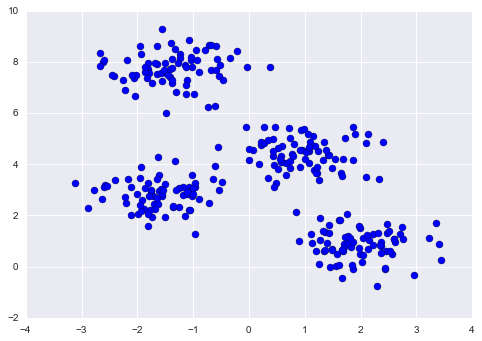
\includegraphics[width=\textwidth]{figs/kmeans-1.png}
 	   \column{.5\textwidth}
       \centering Clustered data\\
		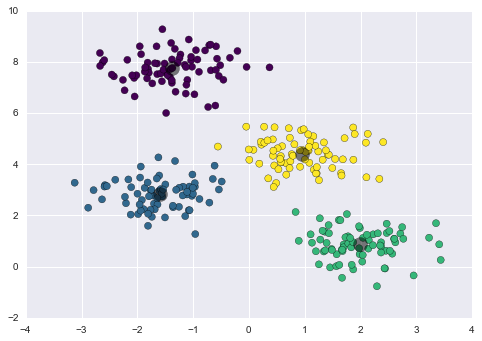
\includegraphics[width=\textwidth]{figs/kmeans-2.png}
    \end{columns}

    \centering \tiny{\href{https://jakevdp.github.io/PythonDataScienceHandbook/05.11-k-means.html}{(Source)}}

    \normalsize
    \begin{flushleft}
    In k-means, clusters are identified by a \alert{centroid}
    \end{flushleft}
\end{frame}


\begin{frame}[fragile]{Algorithms}{K-means (III)}
    K-means drawbacks
    \begin{itemize}
        \item Initial seed
        \item K election
    \end{itemize}

    \begin{columns}
 	   \column{.50\textwidth}
        \begin{block}{Elbow method}
           \begin{enumerate}
            \item Select $K=1, ..., n$
            \item Visualize performance for each k
            \item Choose K where metric stabilizes
           \end{enumerate} 
        \end{block}
 	   \column{.50\textwidth}
			\begin{figure}
		        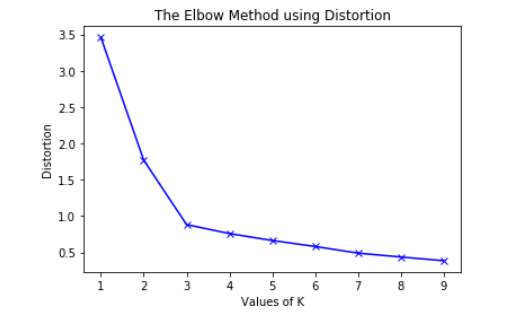
\includegraphics[width=\textwidth]{figs/elbow.png}
			\end{figure}
    \end{columns}

\end{frame}

\subsection{GMM}

\begin{frame}{Algorithms}{Gaussian Mixure Model (GMM)}
	GMM builds a probabilic model of our data
	\begin{itemize}
		\item GMM is a generative clustering algorithm
		\item Assumes data coming from a set of multidimensional gaussian distributions
			\begin{itemize}
				\item GMM fits a set $\{(\mu_i, \sigma_i)\}_{i=1,\dots, K}$
				\item $\mu$ is a vector
				\item $\sigma$ is a covariance matrix
			\end{itemize}
	\end{itemize}

	\bigskip
	\centering 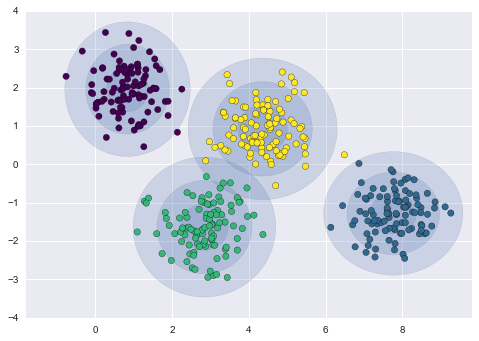
\includegraphics[width=0.31\linewidth]{figs/gmm2.png}
	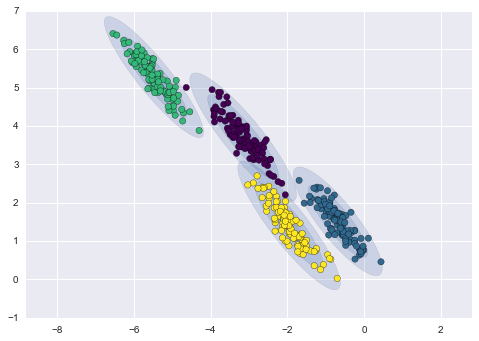
\includegraphics[width=0.31\linewidth]{figs/gmm3.png}
	\centering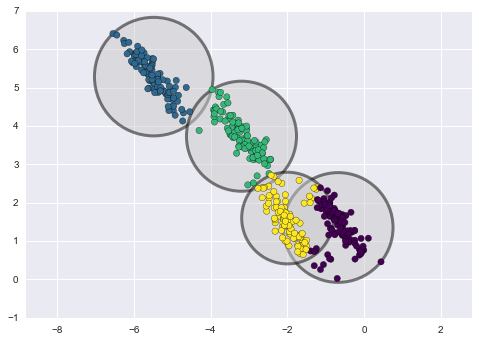
\includegraphics[width=0.31\linewidth]{figs/gmm1.png}\\
	\scriptsize\href{https://jakevdp.github.io/PythonDataScienceHandbook/05.12-gaussian-mixtures.html}{(Source)}
\end{frame}

\subsection{PCA}

\begin{frame}{Algorithms}{Principal Components Analysis (I)}
	Dimensionality reduction transforms data into more convenient representations
	\begin{itemize}
		\item Reduce data dimensionality
		\item Visualize multidimensional data
	\end{itemize}

	Main algorithms
	\begin{itemize}
		\item Isomap
		\item T-distributed Stochastic Neighbor Embedding (t-SNE)
		\item Principal Components Analysis (PCA)
	\end{itemize}

\end{frame}

\begin{frame}{Algorithms}{Principal Components Analysis (II)}
	PCA maximizes data variance

    \begin{columns}
 	   \column{.50\textwidth}
			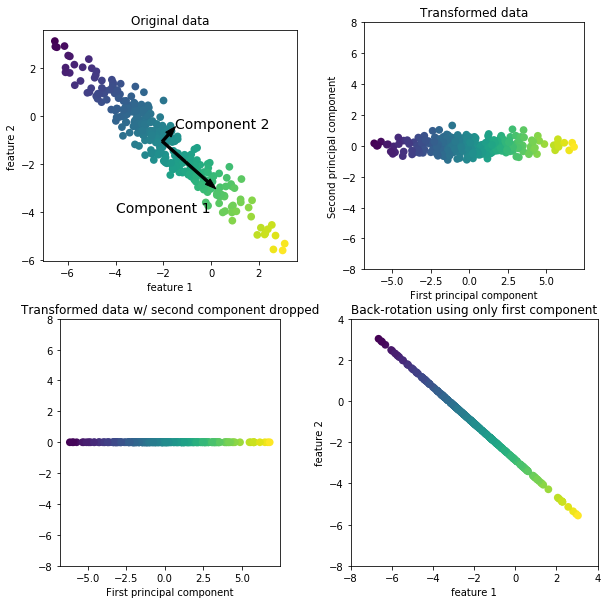
\includegraphics[width=\linewidth]{figs/pca.png}
    		\centering \tiny{\href{https://github.com/amueller/introduction_to_ml_with_python/blob/master/03-unsupervised-learning.ipynb}{(Source)}}
    \end{columns}
\end{frame}

\begin{frame}{Algorithms}{Principal Components Analysis (III)}
	\vspace{-0.5cm}
    \begin{columns}
 	   \column{.70\textwidth}
		Example: Hand-written digits recognition
		\begin{itemize}
			\item Images of hand-written digits
			\item 8x8 images (64 dimensions)
			\item $10$ digits
			\item Classification problem
		\end{itemize}
 	   \column{.30\textwidth}
			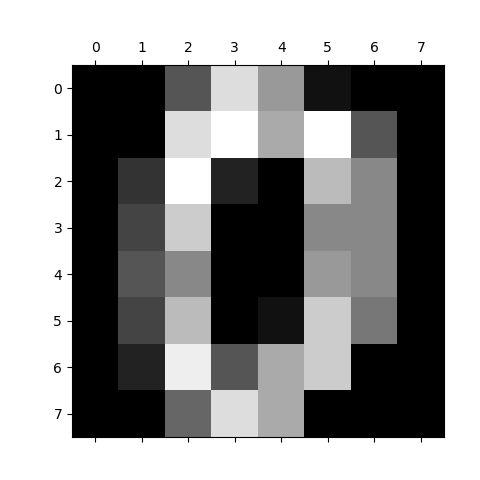
\includegraphics[width=\linewidth]{figs/zero.png}
    \end{columns}

    \begin{columns}
 	   \column{.50\textwidth}
			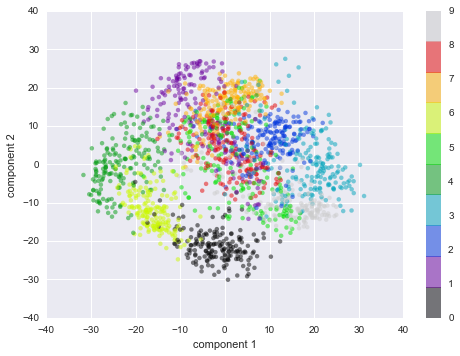
\includegraphics[width=\linewidth]{figs/handdigitspca.png}
 	   \column{.50\textwidth}
			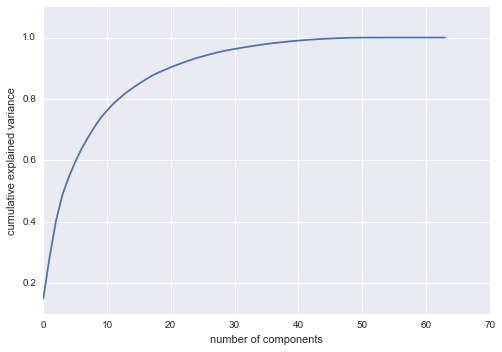
\includegraphics[width=\linewidth]{figs/pcacomponents.png}
    \end{columns}

   	\centering \tiny{\href{https://github.com/amueller/introduction_to_ml_with_python/blob/master/03-unsupervised-learning.ipynb}{(Source)}}
\end{frame}



\end{document}
